\documentclass{article}\usepackage[]{graphicx}\usepackage[]{color}
%% maxwidth is the original width if it is less than linewidth
%% otherwise use linewidth (to make sure the graphics do not exceed the margin)
\makeatletter
\def\maxwidth{ %
  \ifdim\Gin@nat@width>\linewidth
    \linewidth
  \else
    \Gin@nat@width
  \fi
}
\makeatother

\definecolor{fgcolor}{rgb}{0.345, 0.345, 0.345}
\newcommand{\hlnum}[1]{\textcolor[rgb]{0.686,0.059,0.569}{#1}}%
\newcommand{\hlstr}[1]{\textcolor[rgb]{0.192,0.494,0.8}{#1}}%
\newcommand{\hlcom}[1]{\textcolor[rgb]{0.678,0.584,0.686}{\textit{#1}}}%
\newcommand{\hlopt}[1]{\textcolor[rgb]{0,0,0}{#1}}%
\newcommand{\hlstd}[1]{\textcolor[rgb]{0.345,0.345,0.345}{#1}}%
\newcommand{\hlkwa}[1]{\textcolor[rgb]{0.161,0.373,0.58}{\textbf{#1}}}%
\newcommand{\hlkwb}[1]{\textcolor[rgb]{0.69,0.353,0.396}{#1}}%
\newcommand{\hlkwc}[1]{\textcolor[rgb]{0.333,0.667,0.333}{#1}}%
\newcommand{\hlkwd}[1]{\textcolor[rgb]{0.737,0.353,0.396}{\textbf{#1}}}%

\usepackage{framed}
\makeatletter
\newenvironment{kframe}{%
 \def\at@end@of@kframe{}%
 \ifinner\ifhmode%
  \def\at@end@of@kframe{\end{minipage}}%
  \begin{minipage}{\columnwidth}%
 \fi\fi%
 \def\FrameCommand##1{\hskip\@totalleftmargin \hskip-\fboxsep
 \colorbox{shadecolor}{##1}\hskip-\fboxsep
     % There is no \\@totalrightmargin, so:
     \hskip-\linewidth \hskip-\@totalleftmargin \hskip\columnwidth}%
 \MakeFramed {\advance\hsize-\width
   \@totalleftmargin\z@ \linewidth\hsize
   \@setminipage}}%
 {\par\unskip\endMakeFramed%
 \at@end@of@kframe}
\makeatother

\definecolor{shadecolor}{rgb}{.97, .97, .97}
\definecolor{messagecolor}{rgb}{0, 0, 0}
\definecolor{warningcolor}{rgb}{1, 0, 1}
\definecolor{errorcolor}{rgb}{1, 0, 0}
\newenvironment{knitrout}{}{} % an empty environment to be redefined in TeX

\usepackage{alltt}

\title{Is the global temperature increasing?}
\author{Marc Los Huertos}
\date{}
\IfFileExists{upquote.sty}{\usepackage{upquote}}{}
\begin{document}

\maketitle

\section{Introduction}

According the the IPCC, the temperature has been changing about 0.X degrees per XX years -- but how is this value derived? How reliable is the value?  

\subsection{Learning Goals}

For this project, you will evaluate determine if the Earth's temperature has in fact changed, and if so, by how much?

\subsection{Driving Question}

Is my region's climate changing?

How is climate change impacting my community?

\subsection{Public Product}

Narrative Blog...

with professional graphics and statistics.

\subsection{Approach}


\section{Procedures}

\subsection{How is temperature data collected?}

\subsection{How are the data store, curated and checked for quality?}

\section{Data Source}


\subsection{Compressed Files}

\begin{knitrout}
\definecolor{shadecolor}{rgb}{0.969, 0.969, 0.969}\color{fgcolor}\begin{kframe}
\begin{alltt}
\hlcom{# Uncompress the files.}
\hlcom{# ghcnd_all}
\hlkwd{source}\hlstd{(}\hlstr{"summarySE.R"}\hlstd{)}

\hlstd{tarfile} \hlkwb{=} \hlstr{"C:\textbackslash{}\textbackslash{}workspace\textbackslash{}\textbackslash{}GitHub\textbackslash{}\textbackslash{}RTricks\textbackslash{}\textbackslash{}300_Global_Warming\textbackslash{}\textbackslash{}Raw Data\textbackslash{}\textbackslash{}ghcnd_all.tar.gz"}

\hlcom{#ftpsource = ftp://ftp.ncdc.noaa.gov/pub/data/ghcn/v3/ghcnm.tmax.latest.qca.tar.gz}


\hlcom{#ghcnm.tmax.latests.qca.tar.qz}
\hlstd{tarfile} \hlkwb{=} \hlstr{"C:\textbackslash{}\textbackslash{}workspace\textbackslash{}\textbackslash{}GitHub\textbackslash{}\textbackslash{}RTricks\textbackslash{}\textbackslash{}300_Global_Warming\textbackslash{}\textbackslash{}Raw Data\textbackslash{}\textbackslash{}ghcnm.tmax.latest.qca.tar.gz"}
\hlcom{# untar(tarfile)}
\end{alltt}
\end{kframe}
\end{knitrout}


\begin{knitrout}
\definecolor{shadecolor}{rgb}{0.969, 0.969, 0.969}\color{fgcolor}\begin{kframe}
\begin{alltt}
\hlstd{stationfile} \hlkwb{=} \hlstr{"/home/CAMPUS/mwl04747/github/Climate_Change_Narratives/Data/ghcnd-stations.txt"}
\end{alltt}
\end{kframe}
\end{knitrout}

\subsection{Obtain Locations}

\begin{knitrout}
\definecolor{shadecolor}{rgb}{0.969, 0.969, 0.969}\color{fgcolor}\begin{kframe}
\begin{alltt}
\hlcom{# read.table(stationfile, header=F, fill=T, row.names=NULL); head(stations)}
\hlstd{stations} \hlkwb{=} \hlstd{(}\hlkwd{read.fwf}\hlstd{(stationfile,} \hlkwc{fill}\hlstd{=T,} \hlkwc{widths}\hlstd{=} \hlkwd{c}\hlstd{(}\hlnum{11}\hlstd{,} \hlnum{9}\hlstd{,} \hlnum{10}\hlstd{,} \hlnum{7}\hlstd{,} \hlnum{3}\hlstd{,} \hlnum{32}\hlstd{,} \hlnum{3}\hlstd{,} \hlnum{4}\hlstd{,} \hlnum{9}\hlstd{), ))}
\hlkwd{names}\hlstd{(stations)}\hlkwb{=} \hlkwd{c}\hlstd{(}\hlstr{"ID"}\hlstd{,} \hlstr{"LAT"}\hlstd{,} \hlstr{"LONG"}\hlstd{,} \hlstr{"ELEV"}\hlstd{,} \hlstr{"STATE"}\hlstd{,} \hlstr{"NAME"}\hlstd{,} \hlstr{"GSN"}\hlstd{,} \hlstr{"HCN_CRN"}\hlstd{,} \hlstr{"WHOID"}\hlstd{)}

\hlkwd{head}\hlstd{(stations)}
\end{alltt}
\begin{verbatim}
##            ID     LAT     LONG  ELEV STATE
## 1 ACW00011604 17.1167 -61.7833  10.1      
## 2 ACW00011647 17.1333 -61.7833  19.2      
## 3 AE000041196 25.3330  55.5170  34.0      
## 4 AEM00041194 25.2550  55.3640  10.4      
## 5 AEM00041217 24.4330  54.6510  26.8      
## 6 AEM00041218 24.2620  55.6090 264.9      
##                               NAME GSN HCN_CRN WHOID
## 1  ST JOHNS COOLIDGE FLD                          NA
## 2  ST JOHNS                                       NA
## 3  SHARJAH INTER. AIRP             GSN         41196
## 4  DUBAI INTL                                  41194
## 5  ABU DHABI INTL                              41217
## 6  AL AIN INTL                                 41218
\end{verbatim}
\begin{alltt}
\hlkwd{str}\hlstd{(stations)}
\end{alltt}
\begin{verbatim}
## 'data.frame':	100747 obs. of  9 variables:
##  $ ID     : Factor w/ 100747 levels "ACW00011604",..: 1 2 3 4 5 6 7 8 9 10 ...
##  $ LAT    : num  17.1 17.1 25.3 25.3 24.4 ...
##  $ LONG   : num  -61.8 -61.8 55.5 55.4 54.7 ...
##  $ ELEV   : num  10.1 19.2 34 10.4 26.8 ...
##  $ STATE  : Factor w/ 76 levels "   "," AB"," AK",..: 1 1 1 1 1 1 1 1 1 1 ...
##  $ NAME   : Factor w/ 93968 levels " 'S HEERENHOEK                  ",..: 79235 79234 76245 23599 287 949 61012 36770 41695 42069 ...
##  $ GSN    : Factor w/ 3 levels "","   ","GSN": 2 2 3 2 2 2 3 2 2 2 ...
##  $ HCN_CRN: Factor w/ 4 levels "","    "," CRN",..: 2 2 2 2 2 2 2 2 2 2 ...
##  $ WHOID  : num  NA NA 41196 41194 41217 ...
\end{verbatim}
\end{kframe}
\end{knitrout}

Example of data:

AG000060680  22.8000    5.4331 1362.0    TAMANRASSET                    GSN     60680        
         

subsection{Selecting and Example Location}

Here's what the data look like:

ID            1-11   Character
YEAR         12-15   Integer
MONTH        16-17   Integer
ELEMENT      18-21   Character
VALUE1       22-26   Integer
MFLAG1       27-27   Character
QFLAG1       28-28   Character
SFLAG1       29-29   Character
VALUE2       30-34   Integer
MFLAG2       35-35   Character
QFLAG2       36-36   Character
SFLAG2       37-37   Character
  .           .          .
  .           .          .
  .           .          .
VALUE31    262-266   Integer
MFLAG31    267-267   Character
QFLAG31    268-268   Character
SFLAG31    269-269   Character

Arizona, let's chech import process for the sites...
\begin{knitrout}
\definecolor{shadecolor}{rgb}{0.969, 0.969, 0.969}\color{fgcolor}\begin{kframe}
\begin{alltt}
\hlstd{stations[stations}\hlopt{$}\hlstd{ID}\hlopt{==}\hlstr{"US1AZMR0019"}\hlstd{,]}
\end{alltt}
\begin{verbatim}
##                ID     LAT      LONG  ELEV STATE
## 48124 US1AZMR0019 33.5902 -111.9712 418.5    AZ
##                                   NAME GSN HCN_CRN WHOID
## 48124  SCOTTSDALE 8.8 SW                              NA
\end{verbatim}
\begin{alltt}
\hlcom{# head(stations[stations$HCN_CRN==" CRN",])}
\end{alltt}
\end{kframe}
\end{knitrout}

Let's get the arizona data into R

\begin{knitrout}
\definecolor{shadecolor}{rgb}{0.969, 0.969, 0.969}\color{fgcolor}\begin{kframe}
\begin{alltt}
\hlcom{# Read the file}
\hlstd{dlyfile} \hlkwb{=} \hlstr{"/home/CAMPUS/mwl04747/github/Climate_Change_Narratives/AGM00060515"}
\hlstd{test} \hlkwb{=} \hlkwd{read.fwf}\hlstd{(dlyfile,}\hlkwc{widths} \hlstd{=} \hlkwd{c}\hlstd{(}\hlnum{11}\hlstd{,} \hlnum{4}\hlstd{,} \hlnum{2}\hlstd{,} \hlnum{4}\hlstd{,} \hlkwd{rep}\hlstd{(}\hlkwd{c}\hlstd{(}\hlnum{5}\hlstd{,} \hlnum{1}\hlstd{,} \hlnum{1}\hlstd{,} \hlnum{1}\hlstd{),}\hlnum{31}\hlstd{)))}
\end{alltt}


{\ttfamily\noindent\color{warningcolor}{\#\# Warning in file(file, "{}rt"{}): cannot open file '/home/CAMPUS/mwl04747/github/Climate\_Change\_Narratives/AGM00060515': No such file or directory}}

{\ttfamily\noindent\bfseries\color{errorcolor}{\#\# Error in file(file, "{}rt"{}): cannot open the connection}}\begin{alltt}
\hlkwd{str}\hlstd{(test)}
\end{alltt}


{\ttfamily\noindent\bfseries\color{errorcolor}{\#\# Error in str(test): object 'test' not found}}\end{kframe}
\end{knitrout}

\begin{knitrout}
\definecolor{shadecolor}{rgb}{0.969, 0.969, 0.969}\color{fgcolor}\begin{kframe}
\begin{alltt}
\hlcom{# practicing loops}
\hlkwa{for} \hlstd{(year} \hlkwa{in} \hlkwd{c}\hlstd{(}\hlnum{2010}\hlstd{,}\hlnum{2011}\hlstd{,}\hlnum{2012}\hlstd{,}\hlnum{2013}\hlstd{,}\hlnum{2014}\hlstd{,}\hlnum{2015}\hlstd{))\{}
  \hlkwd{print}\hlstd{(}\hlkwd{paste}\hlstd{(}\hlstr{"The year is"}\hlstd{, year))}
\hlstd{\}}
\end{alltt}
\begin{verbatim}
## [1] "The year is 2010"
## [1] "The year is 2011"
## [1] "The year is 2012"
## [1] "The year is 2013"
## [1] "The year is 2014"
## [1] "The year is 2015"
\end{verbatim}
\begin{alltt}
\hlcom{# Create New Varible Names}
\hlstd{MFLAG}\hlkwb{=}\hlnum{NA}\hlstd{; QFLAG}\hlkwb{=}\hlnum{NA}\hlstd{; SFLAG}\hlkwb{=}\hlnum{NA}\hlstd{; VALUE}\hlkwb{=}\hlnum{NA}
\hlkwa{for} \hlstd{(i} \hlkwa{in} \hlnum{1}\hlopt{:}\hlnum{31}\hlstd{)\{}
\hlstd{VALUE[i]} \hlkwb{=} \hlkwd{paste}\hlstd{(}\hlstr{"DATE"}\hlstd{, i,} \hlkwc{sep}\hlstd{=}\hlstr{""}\hlstd{)}
\hlstd{MFLAG[i]} \hlkwb{=} \hlkwd{paste}\hlstd{(}\hlstr{"MFLAG"}\hlstd{, i,} \hlkwc{sep}\hlstd{=}\hlstr{""}\hlstd{)}
\hlstd{QFLAG[i]} \hlkwb{=} \hlkwd{paste}\hlstd{(}\hlstr{"QFLAG"}\hlstd{, i,} \hlkwc{sep}\hlstd{=}\hlstr{""}\hlstd{)}
\hlstd{SFLAG[i]} \hlkwb{=} \hlkwd{paste}\hlstd{(}\hlstr{"SFLAG"}\hlstd{, i,} \hlkwc{sep}\hlstd{=}\hlstr{""}\hlstd{)}
\hlstd{\}}

\hlcom{#print(QFLAG)}



\hlcom{# Vector of variable names converted from a transposed matrix}
\hlstd{tmp} \hlkwb{=} \hlkwd{as.vector}\hlstd{(}\hlkwd{t}\hlstd{(}\hlkwd{matrix}\hlstd{(}\hlkwc{data}\hlstd{=}\hlkwd{c}\hlstd{(VALUE, MFLAG, QFLAG, SFLAG),} \hlkwc{ncol}\hlstd{=}\hlnum{4}\hlstd{)))}
\hlstd{Names} \hlkwb{=} \hlkwd{c}\hlstd{(}\hlstr{"ID"}\hlstd{,} \hlstr{"YEAR"}\hlstd{,} \hlstr{"MONTH"}\hlstd{,} \hlstr{"ELEMENT"}\hlstd{, tmp);} \hlkwd{length}\hlstd{(Names)}
\end{alltt}
\begin{verbatim}
## [1] 128
\end{verbatim}
\begin{alltt}
\hlkwd{names}\hlstd{(test)}\hlkwb{=} \hlstd{Names;} \hlcom{#test}
\end{alltt}


{\ttfamily\noindent\bfseries\color{errorcolor}{\#\# Error in names(test) = Names: object 'test' not found}}\begin{alltt}
\hlkwd{head}\hlstd{(test)}
\end{alltt}


{\ttfamily\noindent\bfseries\color{errorcolor}{\#\# Error in head(test): object 'test' not found}}\end{kframe}
\end{knitrout}

\subsection{Process Selected Data Files}

\begin{knitrout}
\definecolor{shadecolor}{rgb}{0.969, 0.969, 0.969}\color{fgcolor}\begin{kframe}
\begin{alltt}
\hlkwd{setwd}\hlstd{(}\hlstr{"/home/CAMPUS/mwl04747/github/Climate_Change_Narratives/Data"}\hlstd{)}

\hlstd{dly_list} \hlkwb{=} \hlkwd{list.files}\hlstd{(}\hlkwc{pattern}\hlstd{=}\hlstr{"*.dly"}\hlstd{);} \hlkwd{head}\hlstd{(dly_list)}
\end{alltt}
\begin{verbatim}
## [1] "AGM00060515.dly" "US1AZCN0021.dly"
\end{verbatim}
\begin{alltt}
\hlcom{#for (i in 1:length(dly_list)) }
\hlkwa{for} \hlstd{(i} \hlkwa{in} \hlnum{1}\hlopt{:}\hlnum{1}\hlstd{)\{}
\hlstd{tmp} \hlkwb{<-} \hlkwd{read.fwf}\hlstd{(dly_list[i],} \hlkwc{widths} \hlstd{=} \hlkwd{c}\hlstd{(}\hlnum{11}\hlstd{,} \hlnum{4}\hlstd{,} \hlnum{2}\hlstd{,} \hlnum{4}\hlstd{,} \hlkwd{rep}\hlstd{(}\hlkwd{c}\hlstd{(}\hlnum{5}\hlstd{,} \hlnum{1}\hlstd{,} \hlnum{1}\hlstd{,} \hlnum{1}\hlstd{),}\hlnum{31}\hlstd{)))}
\hlkwd{names}\hlstd{(tmp)} \hlkwb{<-} \hlstd{Names}
\hlkwd{assign}\hlstd{(dly_list[i],} \hlkwd{subset}\hlstd{(tmp, ELEMENT}\hlopt{==}\hlstr{"TMAX"}\hlstd{,} \hlkwc{select}\hlstd{=}\hlkwd{c}\hlstd{(}\hlnum{1}\hlopt{:}\hlnum{4}\hlstd{,} \hlkwd{seq}\hlstd{(}\hlnum{5}\hlstd{,} \hlkwc{by} \hlstd{=} \hlnum{4}\hlstd{,} \hlkwc{length.out}\hlstd{=}\hlnum{31}\hlstd{))))}
\hlstd{\}}

\hlkwd{library}\hlstd{(tidyr)}
\hlkwd{library}\hlstd{(dplyr)}
\end{alltt}


{\ttfamily\noindent\itshape\color{messagecolor}{\#\# \\\#\# Attaching package: 'dplyr'\\\#\# \\\#\# The following objects are masked from 'package:stats':\\\#\# \\\#\#\ \ \ \  filter, lag\\\#\# \\\#\# The following objects are masked from 'package:base':\\\#\# \\\#\#\ \ \ \  intersect, setdiff, setequal, union}}\begin{alltt}
\hlkwd{library}\hlstd{(stringr)}
\hlcom{#str(AGM00060515.dly)}
\hlcom{#gather(US1AZCN0021.dly, "Temp", VALUE1)}

\hlkwd{library}\hlstd{(reshape2)}
\hlstd{tmp1} \hlkwb{=} \hlkwd{melt}\hlstd{(AGM00060515.dly,} \hlkwc{id}\hlstd{=}\hlkwd{c}\hlstd{(}\hlstr{"ID"}\hlstd{,} \hlstr{"YEAR"}\hlstd{,} \hlstr{"MONTH"}\hlstd{,} \hlstr{"ELEMENT"}\hlstd{))}
\hlkwd{head}\hlstd{(tmp1)}
\end{alltt}
\begin{verbatim}
##            ID YEAR MONTH ELEMENT variable value
## 1 AGM00060515 1984     3    TMAX    DATE1 -9999
## 2 AGM00060515 1984     4    TMAX    DATE1   190
## 3 AGM00060515 1984     5    TMAX    DATE1 -9999
## 4 AGM00060515 1984     6    TMAX    DATE1 -9999
## 5 AGM00060515 1984     7    TMAX    DATE1   430
## 6 AGM00060515 1984     8    TMAX    DATE1 -9999
\end{verbatim}
\begin{alltt}
\hlstd{tmp1}\hlopt{$}\hlstd{Day} \hlkwb{=} \hlkwd{as.numeric}\hlstd{(}\hlkwd{str_sub}\hlstd{(tmp1}\hlopt{$}\hlstd{variable,}\hlnum{6}\hlstd{,}\hlnum{7}\hlstd{));} \hlkwd{head}\hlstd{(tmp1)}
\end{alltt}
\begin{verbatim}
##            ID YEAR MONTH ELEMENT variable value Day
## 1 AGM00060515 1984     3    TMAX    DATE1 -9999  NA
## 2 AGM00060515 1984     4    TMAX    DATE1   190  NA
## 3 AGM00060515 1984     5    TMAX    DATE1 -9999  NA
## 4 AGM00060515 1984     6    TMAX    DATE1 -9999  NA
## 5 AGM00060515 1984     7    TMAX    DATE1   430  NA
## 6 AGM00060515 1984     8    TMAX    DATE1 -9999  NA
\end{verbatim}
\begin{alltt}
\hlstd{tmp1}\hlopt{$}\hlstd{value[tmp1}\hlopt{$}\hlstd{value}\hlopt{==-}\hlnum{9999}\hlstd{]} \hlkwb{=} \hlnum{NA}\hlstd{;} \hlkwd{head}\hlstd{(tmp1)}
\end{alltt}
\begin{verbatim}
##            ID YEAR MONTH ELEMENT variable value Day
## 1 AGM00060515 1984     3    TMAX    DATE1    NA  NA
## 2 AGM00060515 1984     4    TMAX    DATE1   190  NA
## 3 AGM00060515 1984     5    TMAX    DATE1    NA  NA
## 4 AGM00060515 1984     6    TMAX    DATE1    NA  NA
## 5 AGM00060515 1984     7    TMAX    DATE1   430  NA
## 6 AGM00060515 1984     8    TMAX    DATE1    NA  NA
\end{verbatim}
\begin{alltt}
\hlstd{tmp1}\hlopt{$}\hlstd{Temperature} \hlkwb{=} \hlstd{tmp1}\hlopt{$}\hlstd{value}\hlopt{/}\hlnum{10}

\hlstd{drops} \hlkwb{<-} \hlkwd{c}\hlstd{(}\hlstr{"variable"}\hlstd{,}\hlstr{"value"}\hlstd{)}
\hlstd{tmp1} \hlkwb{<-}\hlstd{tmp1[ ,} \hlopt{!}\hlstd{(}\hlkwd{names}\hlstd{(tmp1)} \hlopt \hlstd{drops)]}
\hlstd{tmp1}\hlopt{$}\hlstd{DECADE} \hlkwb{=} \hlkwd{round}\hlstd{(tmp1}\hlopt{$}\hlstd{YEAR,} \hlopt{-}\hlnum{1}\hlstd{)}
\hlcom{# names(tmp1)}
\end{alltt}
\end{kframe}
\end{knitrout}


\section{Presenting the Results}

\begin{knitrout}
\definecolor{shadecolor}{rgb}{0.969, 0.969, 0.969}\color{fgcolor}\begin{kframe}
\begin{alltt}
\hlcom{# call summarySE function....somehow...}


\hlkwd{library}\hlstd{(ggplot2)}

\hlstd{summarydf} \hlkwb{<-} \hlkwd{summarySE}\hlstd{(tmp1,} \hlstr{"Temperature"}\hlstd{,} \hlstr{"DECADE"}\hlstd{,} \hlkwc{na.rm}\hlstd{=T)}
\end{alltt}


{\ttfamily\noindent\itshape\color{messagecolor}{\#\# -------------------------------------------------------------------------\\\#\# You have loaded plyr after dplyr - this is likely to cause problems.\\\#\# If you need functions from both plyr and dplyr, please load plyr first, then dplyr:\\\#\# library(plyr); library(dplyr)\\\#\# -------------------------------------------------------------------------\\\#\# \\\#\# Attaching package: 'plyr'\\\#\# \\\#\# The following objects are masked from 'package:dplyr':\\\#\# \\\#\#\ \ \ \  arrange, count, desc, failwith, id, mutate, rename, summarise,\\\#\#\ \ \ \  summarize}}\begin{alltt}
\hlkwd{ggplot}\hlstd{(summarydf,} \hlkwd{aes}\hlstd{(}\hlkwc{y}\hlstd{=Temperature,} \hlkwc{x}\hlstd{=DECADE,} \hlkwc{color}\hlstd{= DECADE))}
\end{alltt}
\end{kframe}
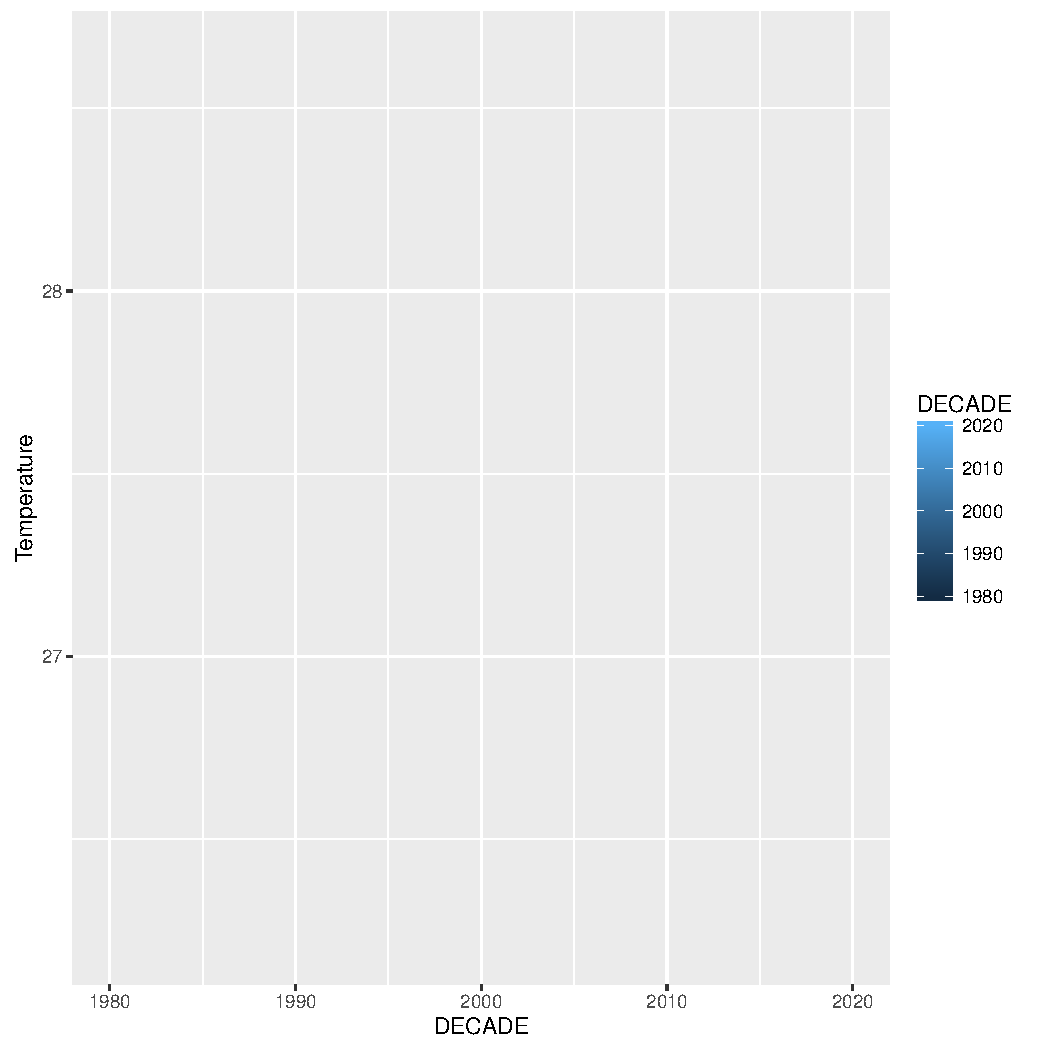
\includegraphics[width=\maxwidth]{figure/unnamed-chunk-6-1} 
\begin{kframe}\begin{alltt}
\hlopt{+} \hlkwd{geom_point}\hlstd{()} \hlopt{+} \hlkwd{geom_errorbar}\hlstd{(limits,} \hlkwc{width}\hlstd{=}\hlnum{0.2}\hlstd{)}
\end{alltt}


{\ttfamily\noindent\bfseries\color{errorcolor}{\#\# Error in +geom\_point(): invalid argument to unary operator}}\begin{alltt}
\hlkwd{ggplot}\hlstd{(summarydf,} \hlkwd{aes}\hlstd{(}\hlkwc{y}\hlstd{=Temperature,} \hlkwc{x}\hlstd{=DECADE,} \hlkwc{color}\hlstd{= DECADE))} \hlopt{+} \hlkwd{geom_errorbar}\hlstd{(}\hlkwd{aes}\hlstd{(}\hlkwc{ymin}\hlstd{=Temperature}\hlopt{-}\hlstd{se,} \hlkwc{ymax}\hlstd{=Temperature}\hlopt{+}\hlstd{se),} \hlkwc{width}\hlstd{=}\hlnum{.2}\hlstd{)} \hlopt{+} \hlkwd{geom_line}\hlstd{()} \hlopt{+} \hlkwd{geom_point}\hlstd{()}
\end{alltt}
\end{kframe}
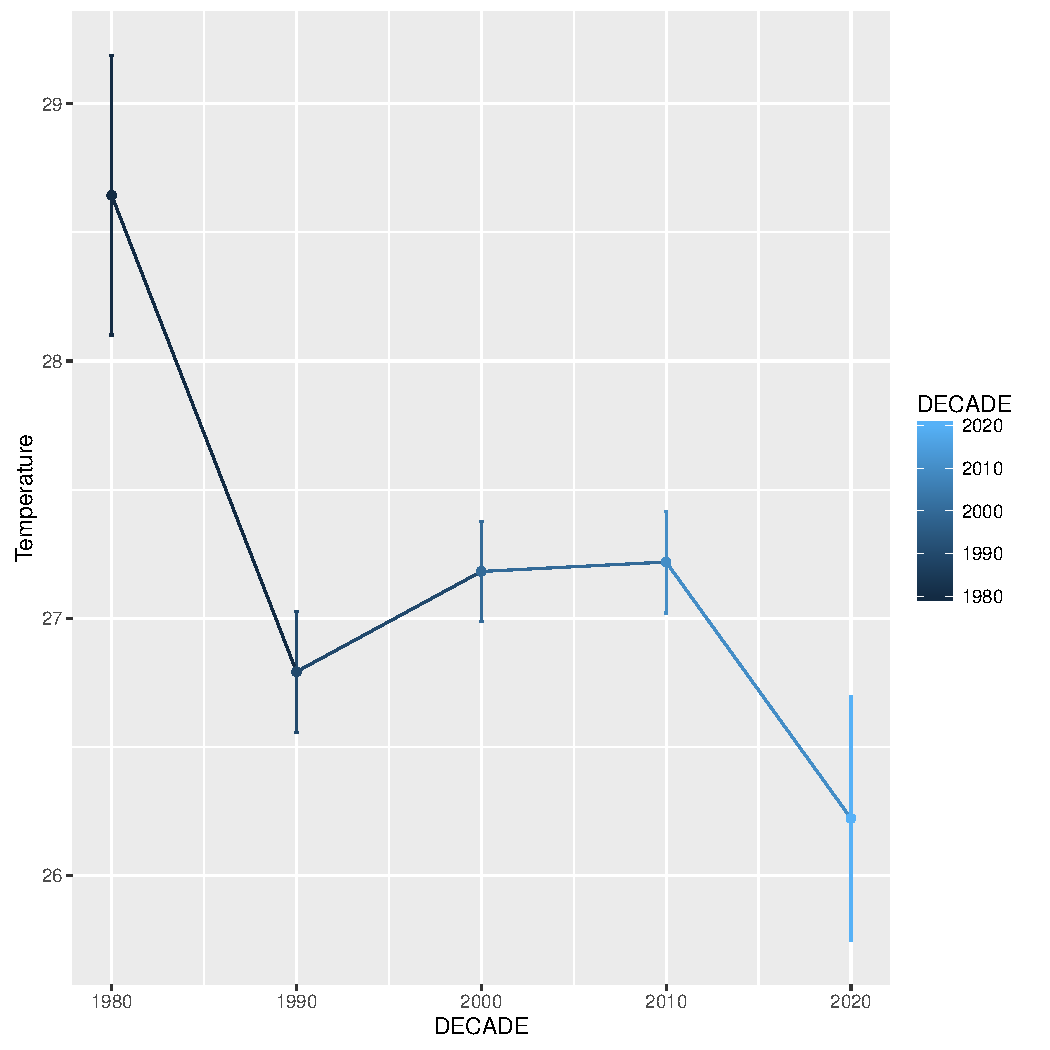
\includegraphics[width=\maxwidth]{figure/unnamed-chunk-6-2} 

\end{knitrout}


%http://www.r-bloggers.com/accessing-cleaning-and-plotting-noaa-temperature-data/


\subsection{NOAA dataset}

New NOAA Directory -- ftp://ftp.ncdc.noaa.gov/pub/data/noaa/

\begin{knitrout}
\definecolor{shadecolor}{rgb}{0.969, 0.969, 0.969}\color{fgcolor}\begin{kframe}
\begin{alltt}
\hlkwd{library}\hlstd{(raster)}
\end{alltt}


{\ttfamily\noindent\itshape\color{messagecolor}{\#\# Loading required package: sp\\\#\# \\\#\# Attaching package: 'raster'\\\#\# \\\#\# The following object is masked from 'package:dplyr':\\\#\# \\\#\#\ \ \ \  select\\\#\# \\\#\# The following object is masked from 'package:tidyr':\\\#\# \\\#\#\ \ \ \  extract}}\begin{alltt}
\hlkwd{library}\hlstd{(XML)}

\hlstd{coords.fwt} \hlkwb{<-} \hlkwd{read.fwf}\hlstd{(}\hlstr{"ftp://ftp.ncdc.noaa.gov/pub/data/noaa/isd-history.txt"}\hlstd{,}\hlkwc{widths}\hlstd{=}\hlkwd{c}\hlstd{(}\hlnum{6}\hlstd{,}\hlnum{1}\hlstd{,}\hlnum{5}\hlstd{,}\hlnum{1}\hlstd{,}\hlnum{38}\hlstd{,}\hlnum{7}\hlstd{,}\hlnum{1}\hlstd{,}\hlnum{8}\hlstd{,}\hlnum{9}\hlstd{,}\hlnum{8}\hlstd{,}\hlnum{1}\hlstd{,}\hlnum{8}\hlstd{),}\hlkwc{sep}\hlstd{=}\hlstr{";"}\hlstd{,}\hlkwc{skip}\hlstd{=}\hlnum{22}\hlstd{,}\hlkwc{fill}\hlstd{=T)}
\hlstd{Names} \hlkwb{=} \hlkwd{c}\hlstd{(}\hlstr{"USAF"}\hlstd{,} \hlstr{"X1"}\hlstd{,} \hlstr{"WBAN"}\hlstd{,} \hlstr{"X2"}\hlstd{,} \hlstr{"STATION_NAME"}\hlstd{,} \hlstr{"X3"}\hlstd{,} \hlstr{"CTRY"}\hlstd{,} \hlstr{"X4"}\hlstd{,} \hlstr{"ST"}\hlstd{,} \hlstr{"X5"}\hlstd{,} \hlstr{"CALL"}\hlstd{,} \hlstr{"X6"}\hlstd{,} \hlstr{"LAT"}\hlstd{,} \hlstr{"X7"}\hlstd{,} \hlstr{"LON"}\hlstd{,} \hlstr{"X8"}\hlstd{,} \hlstr{"ELEV"}\hlstd{,} \hlstr{"X9"}\hlstd{,} \hlstr{"BEGIN"}\hlstd{,} \hlstr{"X10"}\hlstd{,} \hlstr{"END"}\hlstd{)}
\hlstd{Widths} \hlkwb{=} \hlkwd{c}\hlstd{(}\hlnum{6}\hlstd{,}       \hlnum{1}\hlstd{,}    \hlnum{5}\hlstd{,}      \hlnum{1}\hlstd{,}        \hlnum{29}\hlstd{,}         \hlnum{1}\hlstd{,}    \hlnum{2}\hlstd{,}      \hlnum{3}\hlstd{,}    \hlnum{2}\hlstd{,}    \hlnum{1}\hlstd{,}    \hlnum{4}\hlstd{,}      \hlnum{1}\hlstd{,}    \hlnum{8}\hlstd{,}     \hlnum{1}\hlstd{,}     \hlnum{8}\hlstd{,}    \hlnum{1}\hlstd{,}    \hlnum{7}\hlstd{,}     \hlnum{1}\hlstd{,}     \hlnum{8}\hlstd{,}      \hlnum{1}\hlstd{,}    \hlnum{8}\hlstd{)}

\hlstd{coords.fwt} \hlkwb{<-} \hlkwd{read.fwf}\hlstd{(}\hlstr{"ftp://ftp.ncdc.noaa.gov/pub/data/noaa/isd-history.txt"}\hlstd{,}\hlkwc{widths}\hlstd{=Widths,}\hlkwc{sep}\hlstd{=}\hlstr{";"}\hlstd{,}\hlkwc{skip}\hlstd{=}\hlnum{22}\hlstd{,}\hlkwc{fill}\hlstd{=T);} \hlkwd{names}\hlstd{(coords.fwt)}\hlkwb{=}\hlstd{Names; coords.fwt[}\hlkwd{c}\hlstd{(}\hlnum{30}\hlstd{,}\hlnum{4000}\hlstd{,}\hlnum{20000}\hlstd{),]}
\end{alltt}
\begin{verbatim}
##         USAF X1  WBAN X2                  STATION_NAME X3 CTRY  X4 ST X5
## 30      8409 NA 99999 NA XM13                                           
## 4000  120010 NA 99999 NA PETROBALTIC BETA                   PL          
## 20000 725292 NA 14976 NA GRINNELL REGIONAL AIRPORT          US     IA   
##       CALL X6    LAT X7     LON X8  ELEV X9    BEGIN X10      END
## 30         NA     NA NA      NA NA    NA NA 20091027  NA 20100104
## 4000       NA 55.467 NA  18.167 NA  46.0 NA 20141127  NA 20141127
## 20000 KGGI NA 41.717 NA -92.700 NA 307.2 NA 20060831  NA 20160628
\end{verbatim}
\begin{alltt}
\hlstd{coords} \hlkwb{<-} \hlkwd{data.frame}\hlstd{(}\hlkwc{ID}\hlstd{=}\hlkwd{paste}\hlstd{(}\hlkwd{as.factor}\hlstd{(coords.fwt[,}\hlnum{1}\hlstd{])),}\hlkwc{WBAN}\hlstd{=}\hlkwd{paste}\hlstd{(}\hlkwd{as.factor}\hlstd{(coords.fwt[,}\hlnum{3}\hlstd{])),}\hlkwc{Lat}\hlstd{=}\hlkwd{as.numeric}\hlstd{(}\hlkwd{paste}\hlstd{(coords.fwt}\hlopt{$}\hlstd{LAT)),}\hlkwc{Lon}\hlstd{=}\hlkwd{as.numeric}\hlstd{(}\hlkwd{paste}\hlstd{(coords.fwt}\hlopt{$}\hlstd{LON)));  coords[}\hlkwd{c}\hlstd{(}\hlnum{30}\hlstd{,}\hlnum{4000}\hlstd{,}\hlnum{20000}\hlstd{),]}
\end{alltt}


{\ttfamily\noindent\color{warningcolor}{\#\# Warning in data.frame(ID = paste(as.factor(coords.fwt[, 1])), WBAN = paste(as.factor(coords.fwt[, : NAs introduced by coercion}}

{\ttfamily\noindent\color{warningcolor}{\#\# Warning in data.frame(ID = paste(as.factor(coords.fwt[, 1])), WBAN = paste(as.factor(coords.fwt[, : NAs introduced by coercion}}\begin{verbatim}
##           ID  WBAN    Lat     Lon
## 30      8409 99999     NA      NA
## 4000  120010 99999 55.467  18.167
## 20000 725292 14976 41.717 -92.700
\end{verbatim}
\end{kframe}
\end{knitrout}

NOAA Locations
\begin{knitrout}
\definecolor{shadecolor}{rgb}{0.969, 0.969, 0.969}\color{fgcolor}\begin{kframe}
\begin{alltt}
\hlkwd{plot}\hlstd{(Lat} \hlopt{~} \hlstd{Lon,} \hlkwc{data}\hlstd{=coords,} \hlkwc{xlim}\hlstd{=}\hlkwd{c}\hlstd{(}\hlopt{-}\hlnum{180}\hlstd{,} \hlnum{180}\hlstd{) )}
\end{alltt}
\end{kframe}
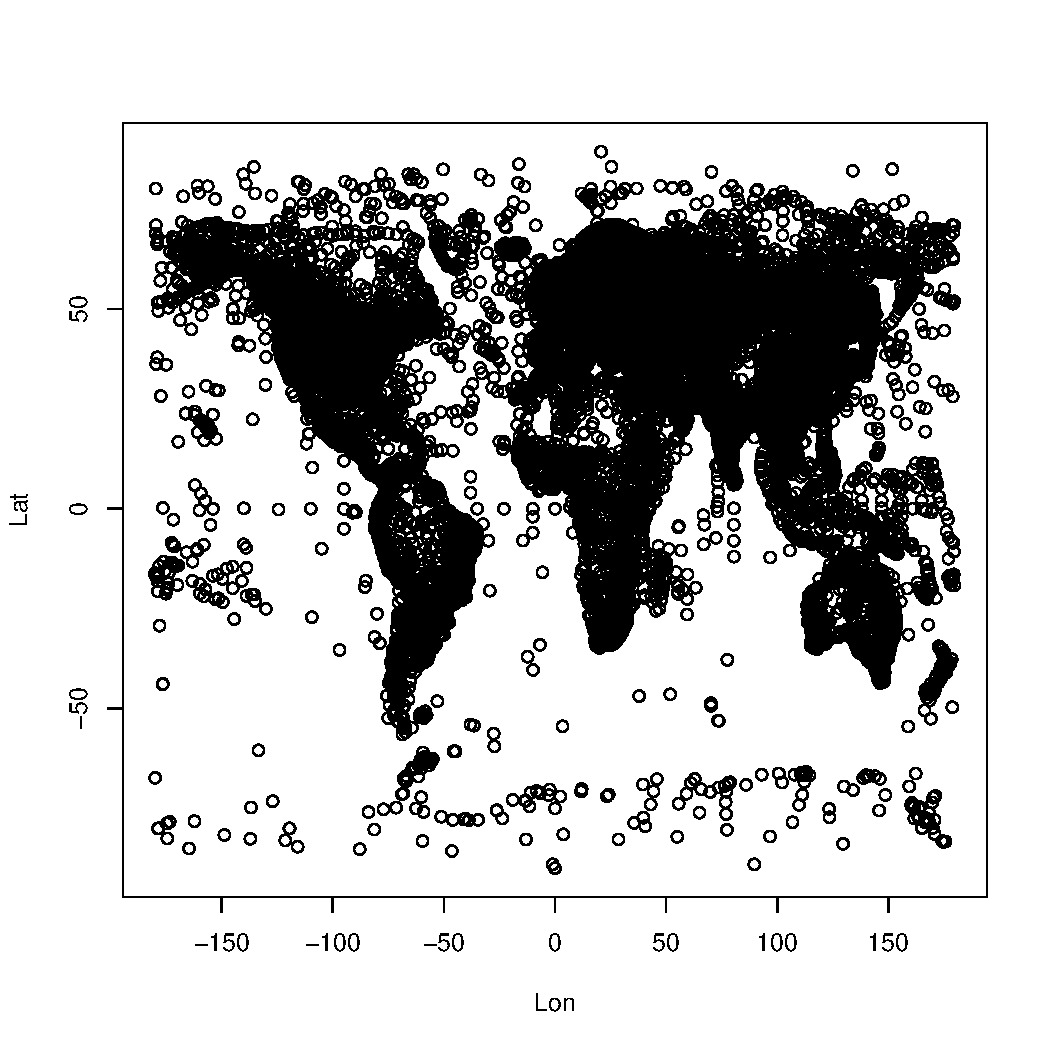
\includegraphics[width=\maxwidth]{figure/NOAApoints-1} 

\end{knitrout}

\end{document}
